
\newcolumntype{M}[1]{>{\centering\arraybackslash}m{#1}}

\begin{table*}[t]
\centering
\caption{
Parameter-sharing strategies in Recursive Transformers. This table shows \textit{Cycle} and \textit{Middle-Cycle} schemes with cyclic layer reuse, where Middle-Cycle retains unique first and last layers. 
}


\label{tab:sharing_strategy}
\renewcommand{\arraystretch}{1.1}
\resizebox{\textwidth}{!}{%
\setlength{\tabcolsep}{7pt}
\begin{tabular}{
    l
  | M{0.32\textwidth} 
  | M{0.16\textwidth} 
  | M{0.32\textwidth} 
  | >{\raggedright\arraybackslash}m{0.16\textwidth} 
}
\toprule
& \multicolumn{2}{c|}{\textbf{Cycle Strategy}} & \multicolumn{2}{c}{\textbf{Middle-Cycle Strategy}}\\
\cmidrule(l{2pt}r{2pt}){2-3}\cmidrule(l{2pt}r{2pt}){4-5}
\textbf{Layers} & Equation & Figure & Equation & \multicolumn{1}{M{0.2\textwidth}}{Figure} \\
\midrule
Last & -- & & $f\bigl(\mathbf{h}_t^{L-1}; \Phi_{L-1}\bigr)$ &\\[14pt]
Recursion & $f\!\Bigl(\mathbf{h}_t^{\ell}; \Phi'_{\ell \bmod (L/N_r)}\Bigr)$ & \multirow{-2}{*}{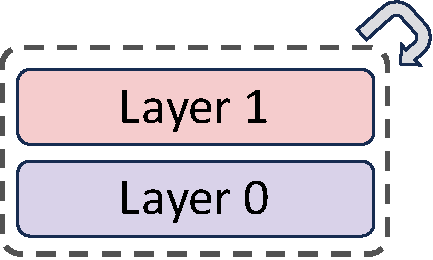
\includegraphics[width=0.91\linewidth]{figs/sharing_strategy/sharing_strategy_cycle.pdf}}
  & $f\!\Bigl(\mathbf{h}_t^{\ell}; \Phi'_{(\ell - 1 \bmod ((L-2)/N_r)) + 1}\Bigr)$ & \multirow{-3}{*}{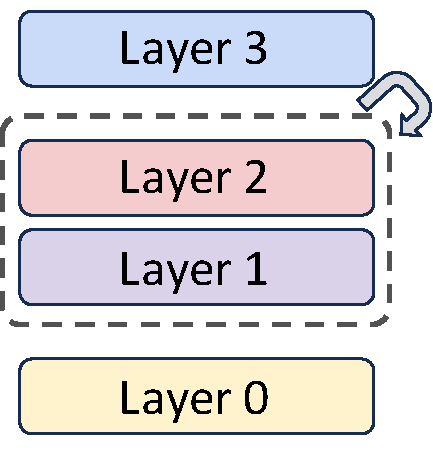
\includegraphics[width=0.91\linewidth]{figs/sharing_strategy/sharing_strategy_middle_cycle.pdf}}  \\[14pt]
First   & --                  &   & $f\bigl(\mathbf{h}_t^{0}; \Phi_0\bigr)$ \\
[4pt]
\bottomrule
\end{tabular}
}
\end{table*}